\documentclass[a4paper,12pt]{article}%

\usepackage{amsmath}
\usepackage{amsfonts}
\usepackage{amssymb}
\usepackage{graphicx}
\usepackage[czech]{babel} %Cestina
\usepackage[cp1250]{inputenc}%hacky, carky
\usepackage{hyperref}
\usepackage{wasysym} %kvuli znacce prumeru
\usepackage{multicol} %umozni vkladat vicesloupcove bloky

%okraje stranky
\usepackage{geometry}
 \geometry{
 a4paper,
 %total={210mm,297mm},
 left=20mm,
 right=20mm,
 top=20mm,
 bottom=20mm,
 }


%-------------------------------------------

\begin{document}

\section{\texorpdfstring{Neline�rn� rezistory}{Nelinearni rezistory}}

\subsection{\texorpdfstring{�vod}{Uvod}}

V praxi se nej�ast�ji setk�v�me s line�rn�mi rezistory, tj. sou��stkami, u nich� p�edpokl�d�me konstantn� velikost odporu nez�vislou na vn�j��ch podm�nk�ch aplikace, tj. nez�vislost na teplot�, frekvenci, mechanick�ch vlivech apod. Odli�uj� se v�konovou zat�itelnost�, teplotn� a frekven�n� z�vislost� podle pou�it�ch materi�l� a  technologi� v�roby, toleranc� jmenovit� hodnoty a proveden�m. P�edpoklad konstantn� velikosti odporu vyhovuje obvykle p�i aplikac�ch do frekvenc� 50~kHz a� 1~MHz (podle proveden�). Pro vy��� frekvence je nutn� uva�ovat �pln� n�hradn� sch�ma rezistoru s jeho reaktan�n�mi prvky.

Neline�rn� rezistory  jsou na rozd�l od line�rn�ch konstruov�ny tak, aby  velikost odporu byla v�razn� z�visl� na vn�j��ch podm�nk�ch, nap�. teplot� (termistory NTC, PTC) nebo p�ilo�en�mu nap�t� (varistory) a pokud mo�no nez�visela na dal��ch vlivech aplikace. Vzhledem k t�mto vlastnostem se vyu��vaj� k m��en� teploty, v obvodech pro tepelnou ochranu p��stroj�, stroj� a za��zen�, jako p�ep�ov� ochrany atd.

%---------------------------------------------
\subsection{\texorpdfstring{M��en� teplotn� z�vislosti termistor�}{Mereni teplotni zavislosti termistoru}}

\subsubsection{\texorpdfstring{�kol m��en�}{Ukol mereni}}
Zm��te z�vislost odporu 6 vzork� rezistor� a termistor� pro zm�nu teploty 20~$^\circ$C a� 120~$^\circ$C. Nam��en� z�vislosti $R= f(\vartheta)$ vyneste do grafu! Ov��te, zda dan� charakteristiky odpov�daj� teoretick�m vztah�m (line�rn� z�vislost, exponenci�ln� z�vislost apod.)

\subsubsection{\texorpdfstring{Sch�ma zapojen�}{Schema zapojeni}}

\begin{figure}[h]
  \centering
  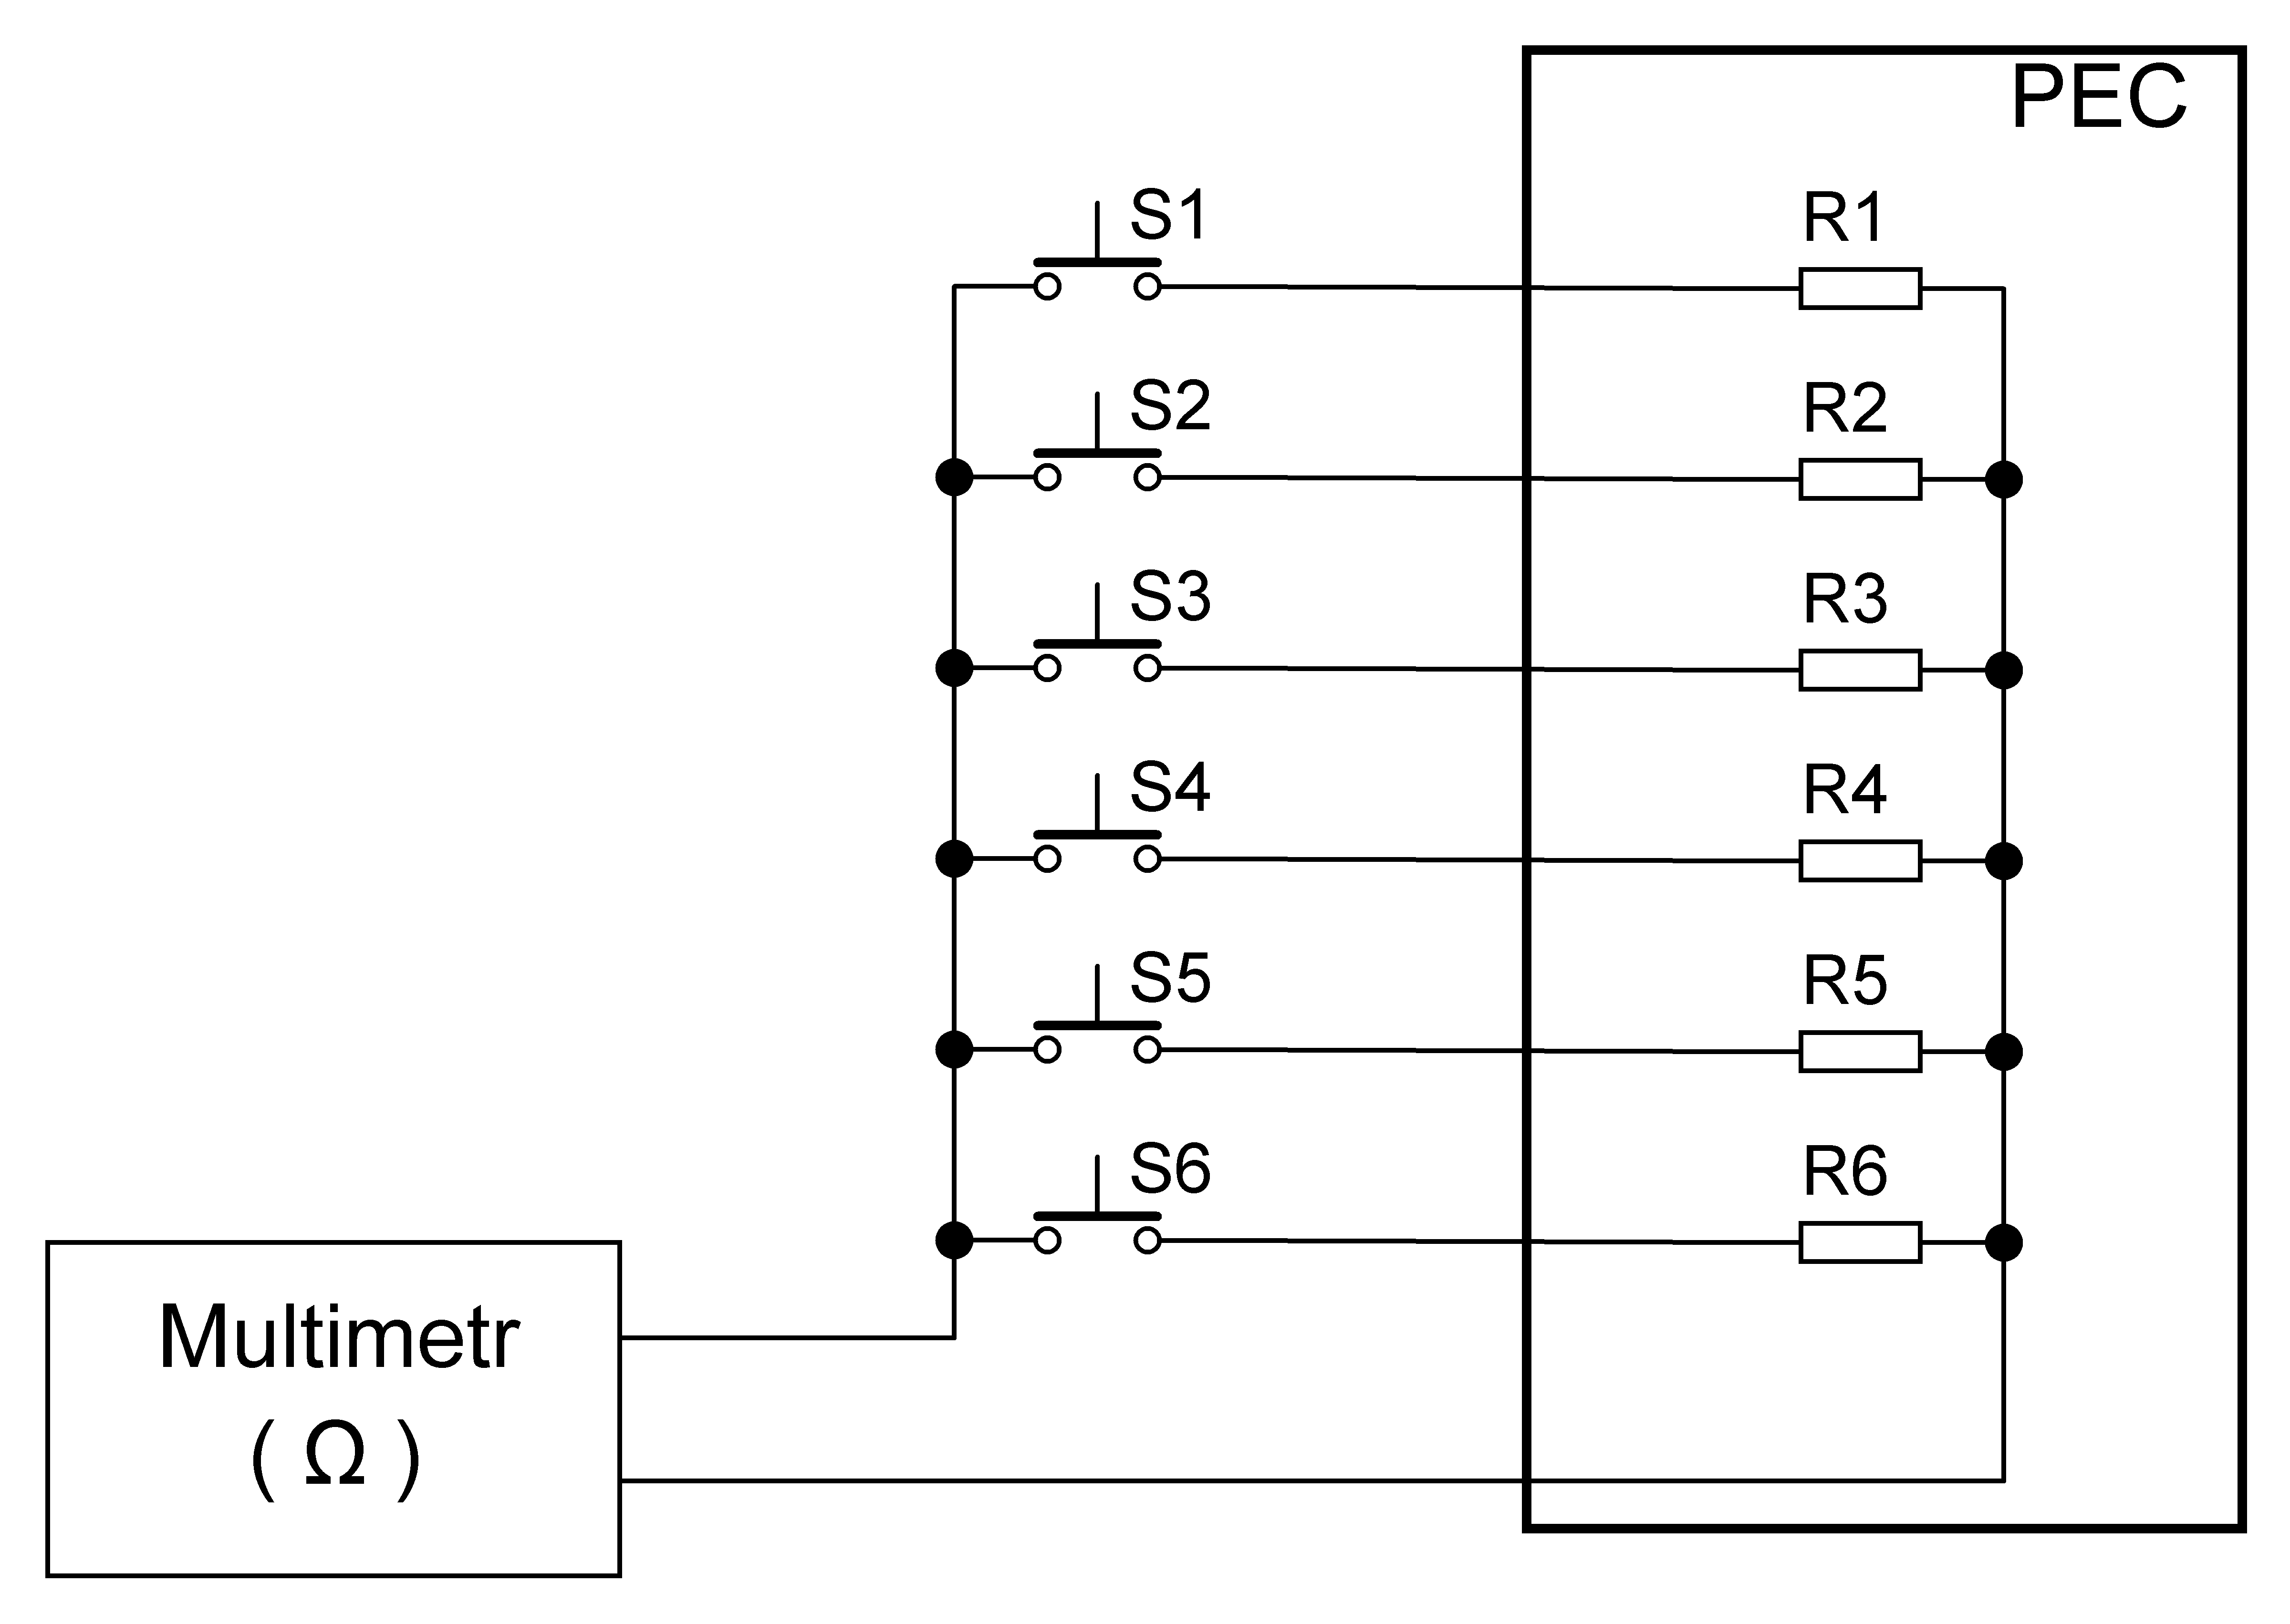
\includegraphics[width=0.5\columnwidth]{nelin_rezistory/NelinRez11}
  \label{fig:nelinRez:termistory}
\end{figure}

\subsubsection{\texorpdfstring{Postup m��en�}{Postup mereni}}

M��en� vzorky jsou um�st�ny na desti�ce v p�cce a vyvedeny na p�ep�na� m��ic�ch m�st. K m��en� teploty slou�� orienta�n� teplom�r, kter� je sou��st� konstrukce pece. Pro p�esn� m��en� vyu�ijeme Pt odporov� teplom�r s line�rn� z�vislost� odporu na teplot�. Pro odpor Pt teplom�ru uva�ujte n�sleduj�c� vztah:

\begin{equation}
R_\vartheta = R_0 \cdot \left(1 + \alpha \cdot\left(\vartheta - \vartheta_0\right)\right)
\label{eq:nelinRez:OdporNaTeplote}
\end{equation}

\begin{tabular}{ll}
 $R_0$& \ldots je odpor v $\Omega$ p�i 0~$^\circ$C, \\
 $\alpha$& \ldots je teplotn� koeficient odporu, pro platinov� teplom�r je $\alpha = 4,5 \cdot 10^{-3}$ K$^{-1}$, \\
 $\vartheta$& \ldots je teplota okol� ve $^\circ$C nebo K, \\ 
 $\vartheta_0$& \ldots je teplota ve $^\circ$C nebo K, p�i kter� byl m��en odpor $R_0$, zde 0~$^\circ$C. \\
\end{tabular}

\subsubsection{\texorpdfstring{M��en� vzorky}{Merene vzorky}}
\begin{tabular}{llll}
 1.& odporov� Pt teplom�r 100~$\Omega$ p�i 0~$^\circ$C&  4.&  rezistor uhl�kov� TR 212  4,7~k$\Omega$  \\
 2.& termistor NTC 100~$\Omega$&  5.& termistor NTC 6,8~k$\Omega$  \\
 3.& rezistor metaloxidov� TR154  6,8~k$\Omega$ &  6.& termistor PTC 60~$\Omega$  \\ 
\end{tabular}

%---------------------------------------------
\subsection{\texorpdfstring{M��en� VA charakteristiky varistor�}{Mereni VA charakteristiky varistoru}}

\subsubsection{\texorpdfstring{�kol m��en�}{Ukol mereni}}
Zm��te voltamp�rovou charakteristiku 5 vzork� varistor� pomoc� osciloskopu, kter� pracuje v re�imu x/y (sou�adnicov� zapisova�). Ov��te, zda �daje uveden� k jednotliv�m vzork�m odpov�daj� m��en�.

\subsubsection{\texorpdfstring{Sch�ma zapojen�}{Schema zapojeni}}

\begin{figure}[h]
  \centering
  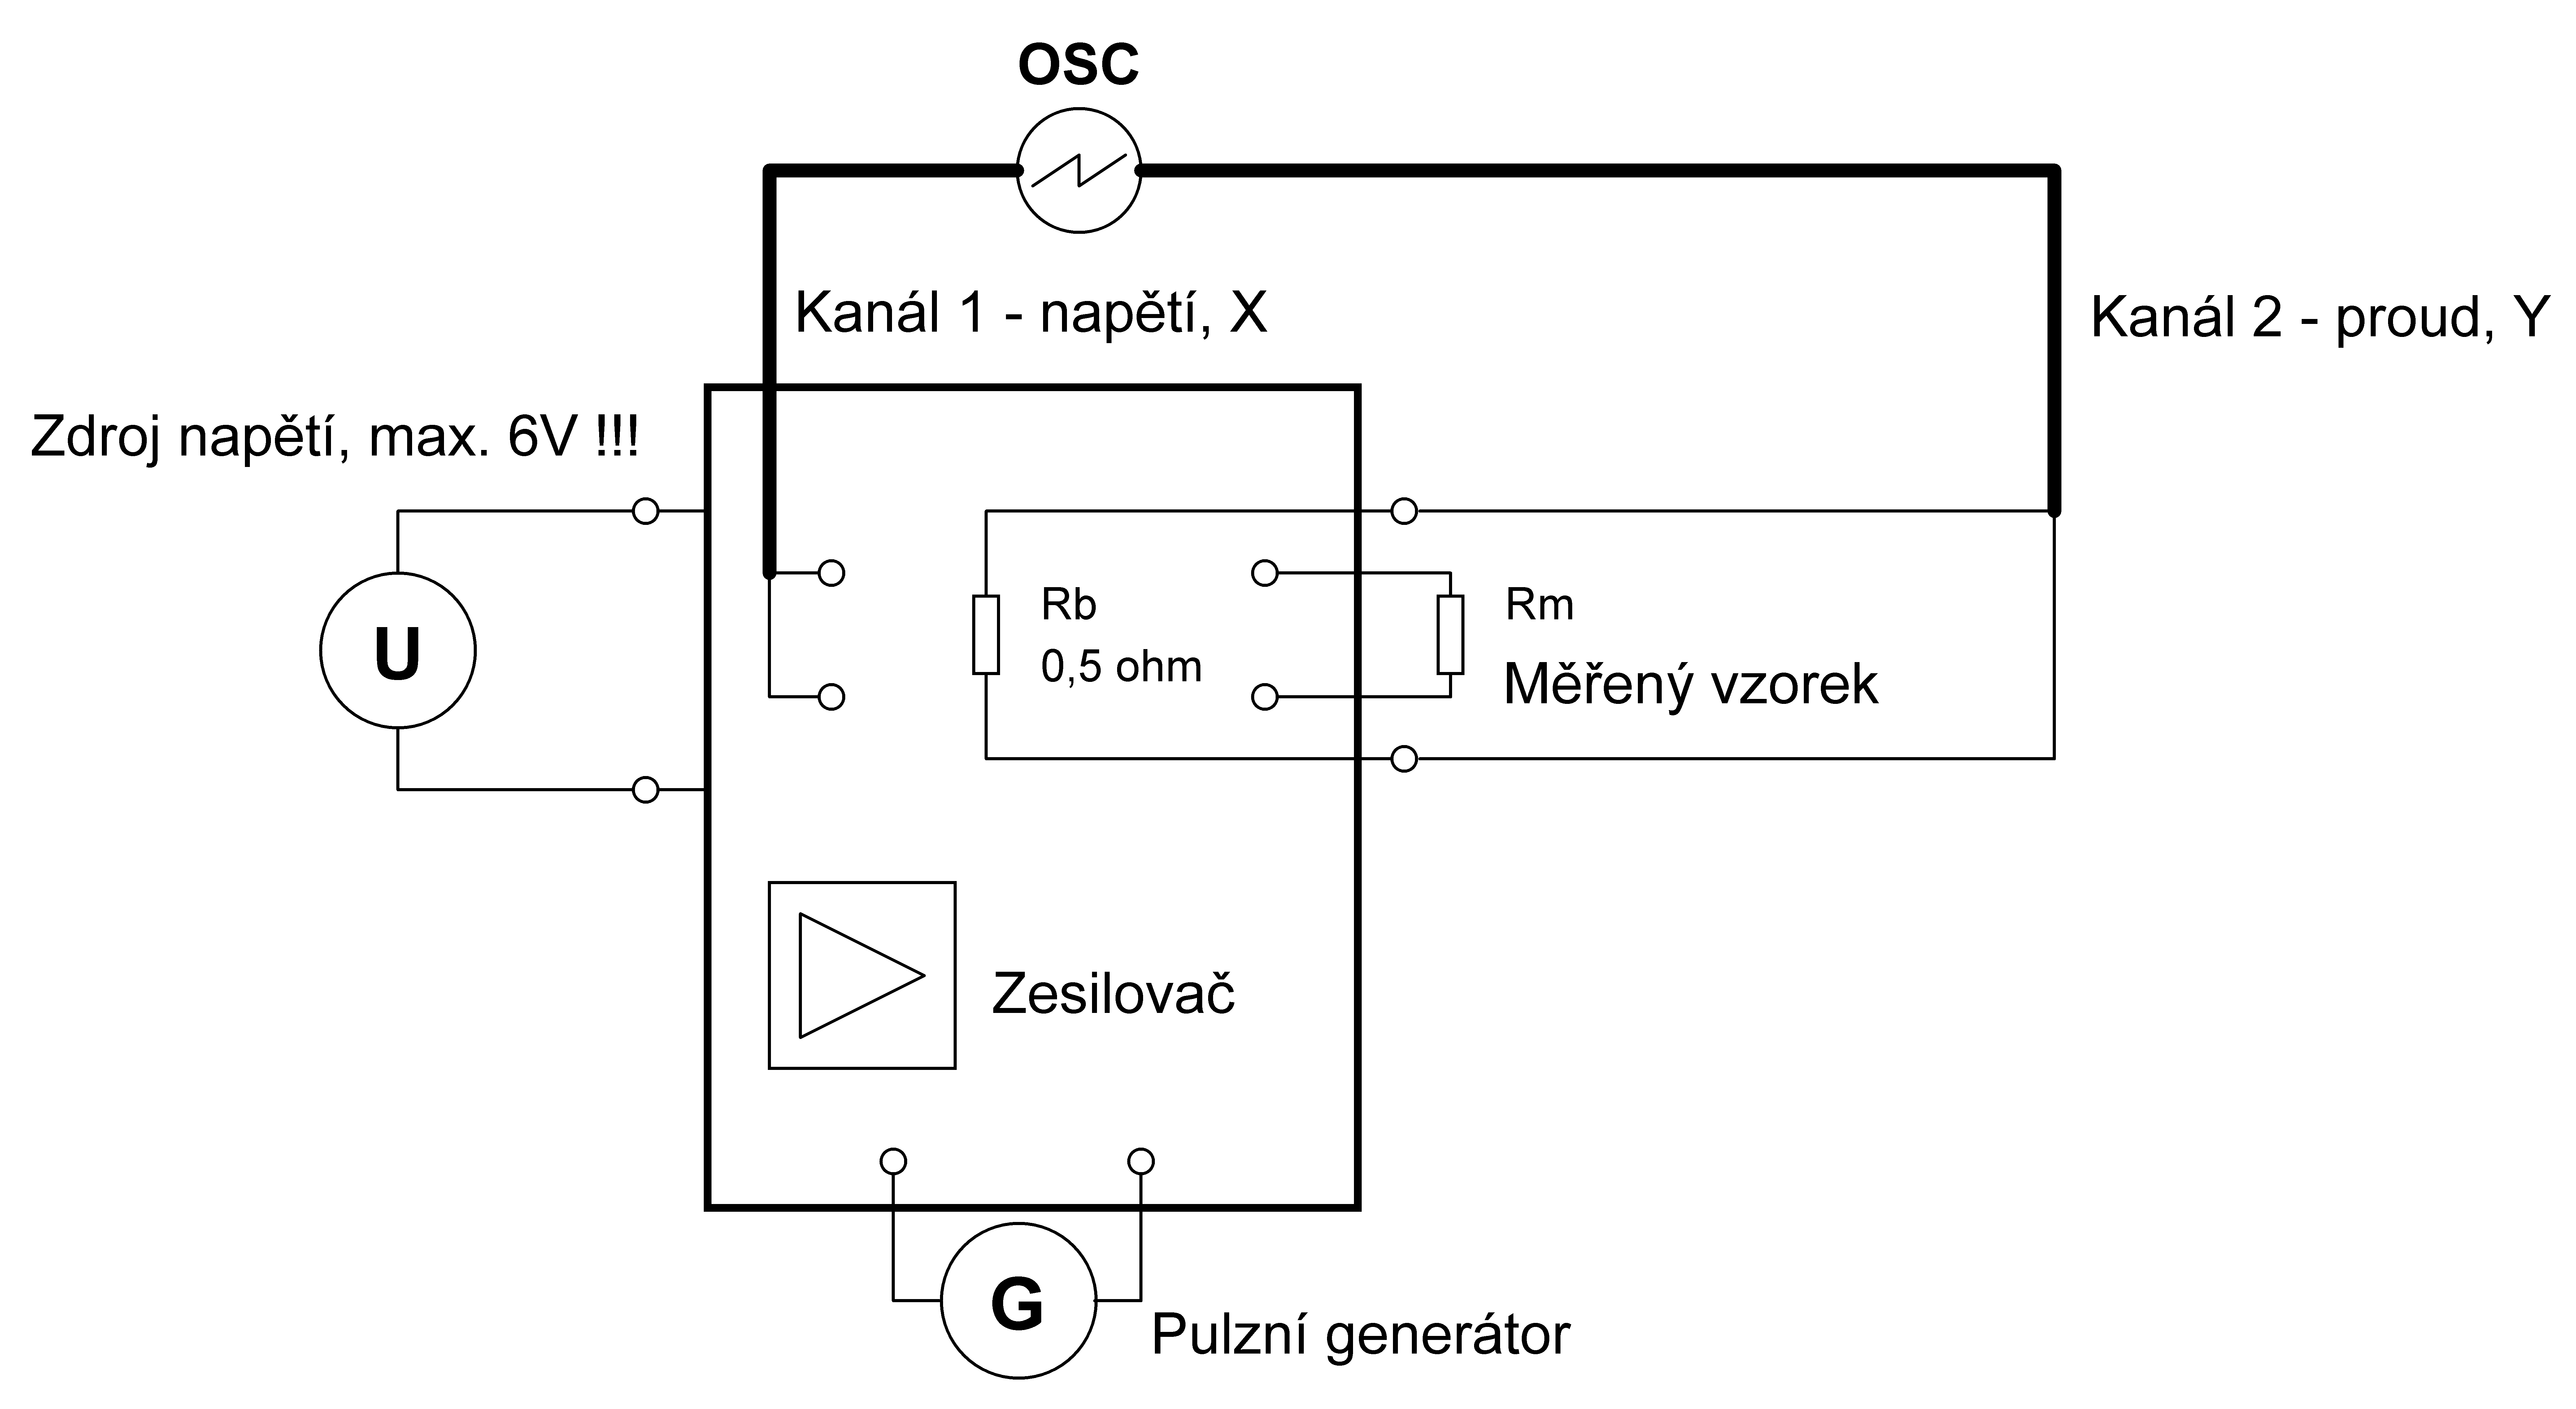
\includegraphics[width=0.8\columnwidth]{nelin_rezistory/NelinRez12}
  \label{fig:nelinRez:varistory}
\end{figure}

\subsubsection{\texorpdfstring{Postup m��en�}{Postup mereni}}

M��en� vzorek um�st�me do p��pravku. Pro m��en� pou�ijeme zdroj kr�tk�ch nap�ov�ch pulz� nastaviteln� velikosti. Pozor p�i v�m�n� vzork� -  p�ed manipulac� sni�te nap�t� na 0~V! Nap�t� na vzorku sn�m�me sondou s d�li�em 1:100 (nastaveno na osciloskopu � zkontrolovat!), proud je sn�m�n jako �bytek nap�t� na odporu 0,5~$\Omega$ nebo pomoc� proudov� sondy.  Sejmut� charakteristiky zaznamenejte na disketu v osciloskopu, p�eneste do PC a ulo�te na vhodn� pam�ov� medium pro vytisknut� do refer�tu z m��en�.

\subsubsection{\texorpdfstring{M��en� vzorky}{Merene vzorky}}
\begin{tabular}{llll}
 1.& 15D201K, 200 V, zelen�&  4.& S20K20, 40 V, velk� modr�  \\
 2.& 14D220K, 22 V, modr�&  5.& TR 152, 100 Ohm�, line�rn� rezistor  \\
 3.& 14D101K, 100 V, sv�tle modr�&  &  \\ 
\end{tabular}
\section{\texorpdfstring{Feroelektrick� kondenz�tory}{Feroelektricke kondenzatory}}

\subsection{\texorpdfstring{�vod}{Uvod}}
Kondenz�tor je sou��stka, pomoc� n� v elektrick�m obvodu realizujeme kapacitu. Podobn� jako ostatn� sou��stky vykazuje �adu vedlej��ch z�vislost� (induk�nost, s�riov� a paraleln� odpor, teplotn� a nap�ovou z�vislost). Hodnota kapacity $C$ z�vis�, jak zn�mo, na plo�e elektrod ($S$), dielektrick� konstant� ($\epsilon$) a nep��mo na vzd�lenosti elektrod ($d$). Z toho vych�zej� odli�n� konstrukce kondenz�tor� (plo�n� - nap�. sl�dov�, svitkov�, keramick�, elektrolytick�). Po�adavek na minim�ln� rozm�ry p�edpokl�d� pou�it� materi�l� dielektrika s vysokou pom�rnou dielektrickou konstantou (tzv. feroelektrika). Tyto materi�ly jsou v�ak p�i vy���ch teplot�ch zna�n� teplotn� z�visl� a jejich $\epsilon_r$ p�i vy��� teplot� rychle kles�.

\subsubsection{\texorpdfstring{Ztr�tov� �initel}{Ztratovy cinitel}}

%--------------------------------------
\newpage
\subsection{\texorpdfstring{M��en� teplotn� z�vislosti kapacity a ztr�tov�ho �initele vybran�ch vzork� kondenz�tor�}{Mereni teplotni zavislosti kapacity a ztratoveho cinitele vybranych vzorku kondenzatoru}}

\subsubsection{\texorpdfstring{�kol m��en�}{Ukol mereni}}
Zm��te z�vislost kapacity $C$ a ztr�tov�ho �initele $D$ u t�� vzork� keramick�ch kondenz�tor� s odli�n�m dielektrikem na teplot� $T$ pro teploty 20~$^\circ$C a� 120~$^\circ$C. Z�vislosti $C = f(T)$, $D = g(T)$ vyneste do grafu.

\subsubsection{\texorpdfstring{Sch�ma zapojen�}{Schema zapojeni}}

\begin{figure}[h]
  \centering
  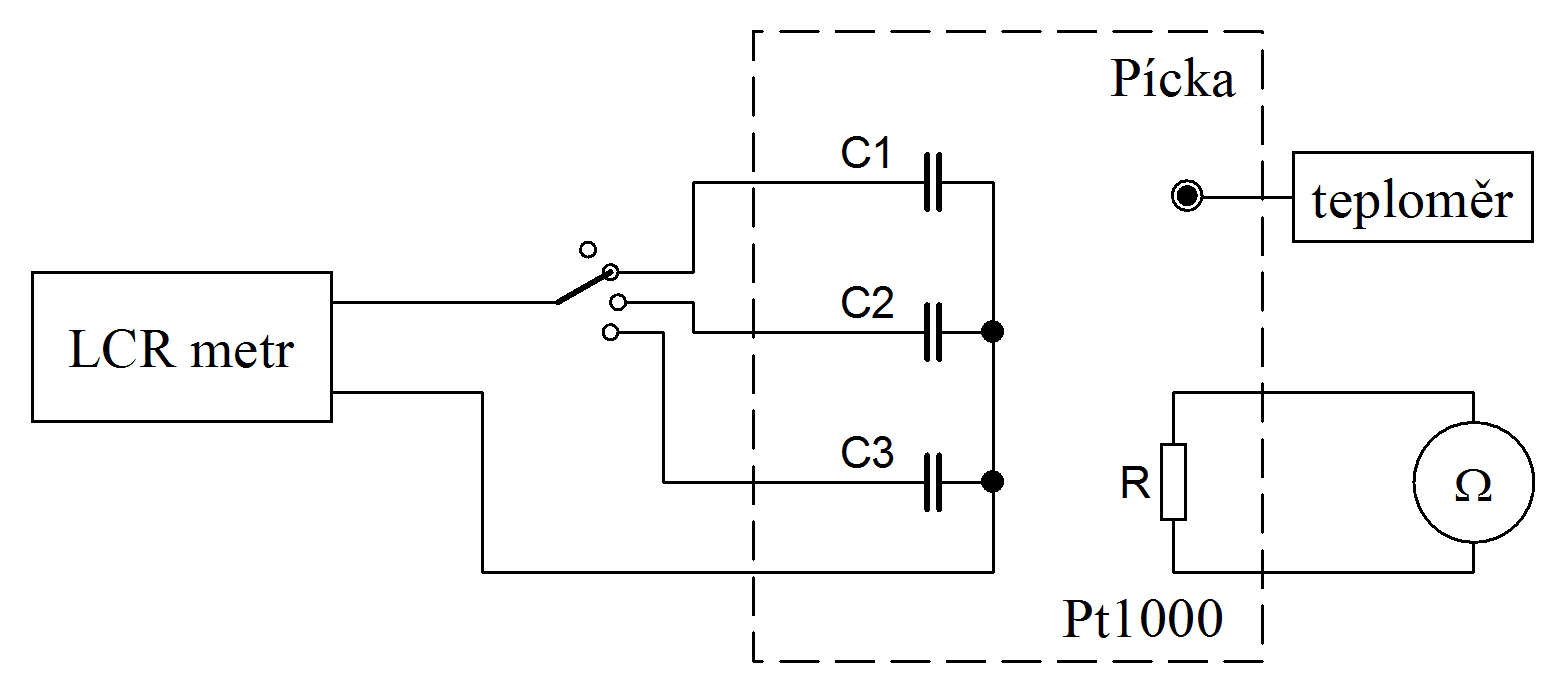
\includegraphics[width=0.7\columnwidth]{feroel_kondenzatory/feroelKond1}
  \label{fig:feroelKond:feroelKond1}
\end{figure}

\subsubsection{\texorpdfstring{Postup m��en�}{Postup mereni}}
M��en� vzorky jsou um�st�ny na desti�ce v p�cce a vyvedeny na p�ep�na� m��ic�ch m�st. K m��en� teploty slou�� orienta�n� dotykov� teplom�r zasazen� do m�rn� j�mky na t�lese p�cky. Kapacitu vzork� a ztr�tov� �initel m���me RLC metrem. K p�esn�mu zm��en� teploty slou�� odporov� teplom�r (�idlo Pt1000, $R_0 = 1008$~$\Omega$ p�i 0~$^\circ$C, $\alpha = 4,5 \cdot 10^{-3}$ K$^{-1}$), jeho� odpor m���me pomoc� multimetru. Teplotu vypo�teme z �daj� uveden�ch v��e v n�vodu a za p�edpokladu linearn� z�vislosti mezi hodnotou odporu a teplotou:
 
\begin{equation}
R_\vartheta = R_0 \cdot \left(1 + \alpha \cdot\left(\vartheta - \vartheta_0\right)\right)
\label{eq:feroelKond:OdporNaTeplote}
\end{equation}

\begin{tabular}{ll}
 $R_0$& \ldots je odpor v $\Omega$ p�i 0~$^\circ$C, \\
 $\alpha$& \ldots je teplotn� koeficient odporu, pro platinov� teplom�r je $\alpha = 4,5 \cdot 10^{-3}$ K$^{-1}$, \\
 $\vartheta$& \ldots je teplota okol� ve $^\circ$C nebo K, \\ 
 $\vartheta_0$& \ldots je teplota ve $^\circ$C nebo K, p�i kter� byl m��en odpor $R_0$, zde 0~$^\circ$C. \\
\end{tabular}

\subsubsection{\texorpdfstring{M��en� vzorky}{Merene vzorky}}
\begin{tabular}{ll}
 1.& keramick� kondenz�tor 100 nF, hmota X7R \\
 2.& keramick� kondenz�tor 150 nF, hmota Z5U \\
 3.& keramick� kondenz�tor 150 nF, hmota Y5VV \\ 
\end{tabular}

%--------------------------------------
\newpage
\subsection{\texorpdfstring{M��en� nap�ov� z�vislosti kapacity vybran�ch vzork� kondenz�tor�}{Mereni napetove zavislosti kapacity vybranych vzorku kondenzatoru}}

\subsubsection{\texorpdfstring{�kol m��en�}{Ukol mereni}}
Zm��te z�vislost kapacity t�� vzork� keramick�ch kondenz�tor� na velikosti p�ilo�en�ho stejnosm�rn�ho nap�t�. Z�vislost $C = f(U)$ vyneste do grafu.

\subsubsection{\texorpdfstring{Sch�ma zapojen�}{Schema zapojeni}}

\begin{figure}[h]
  \centering
  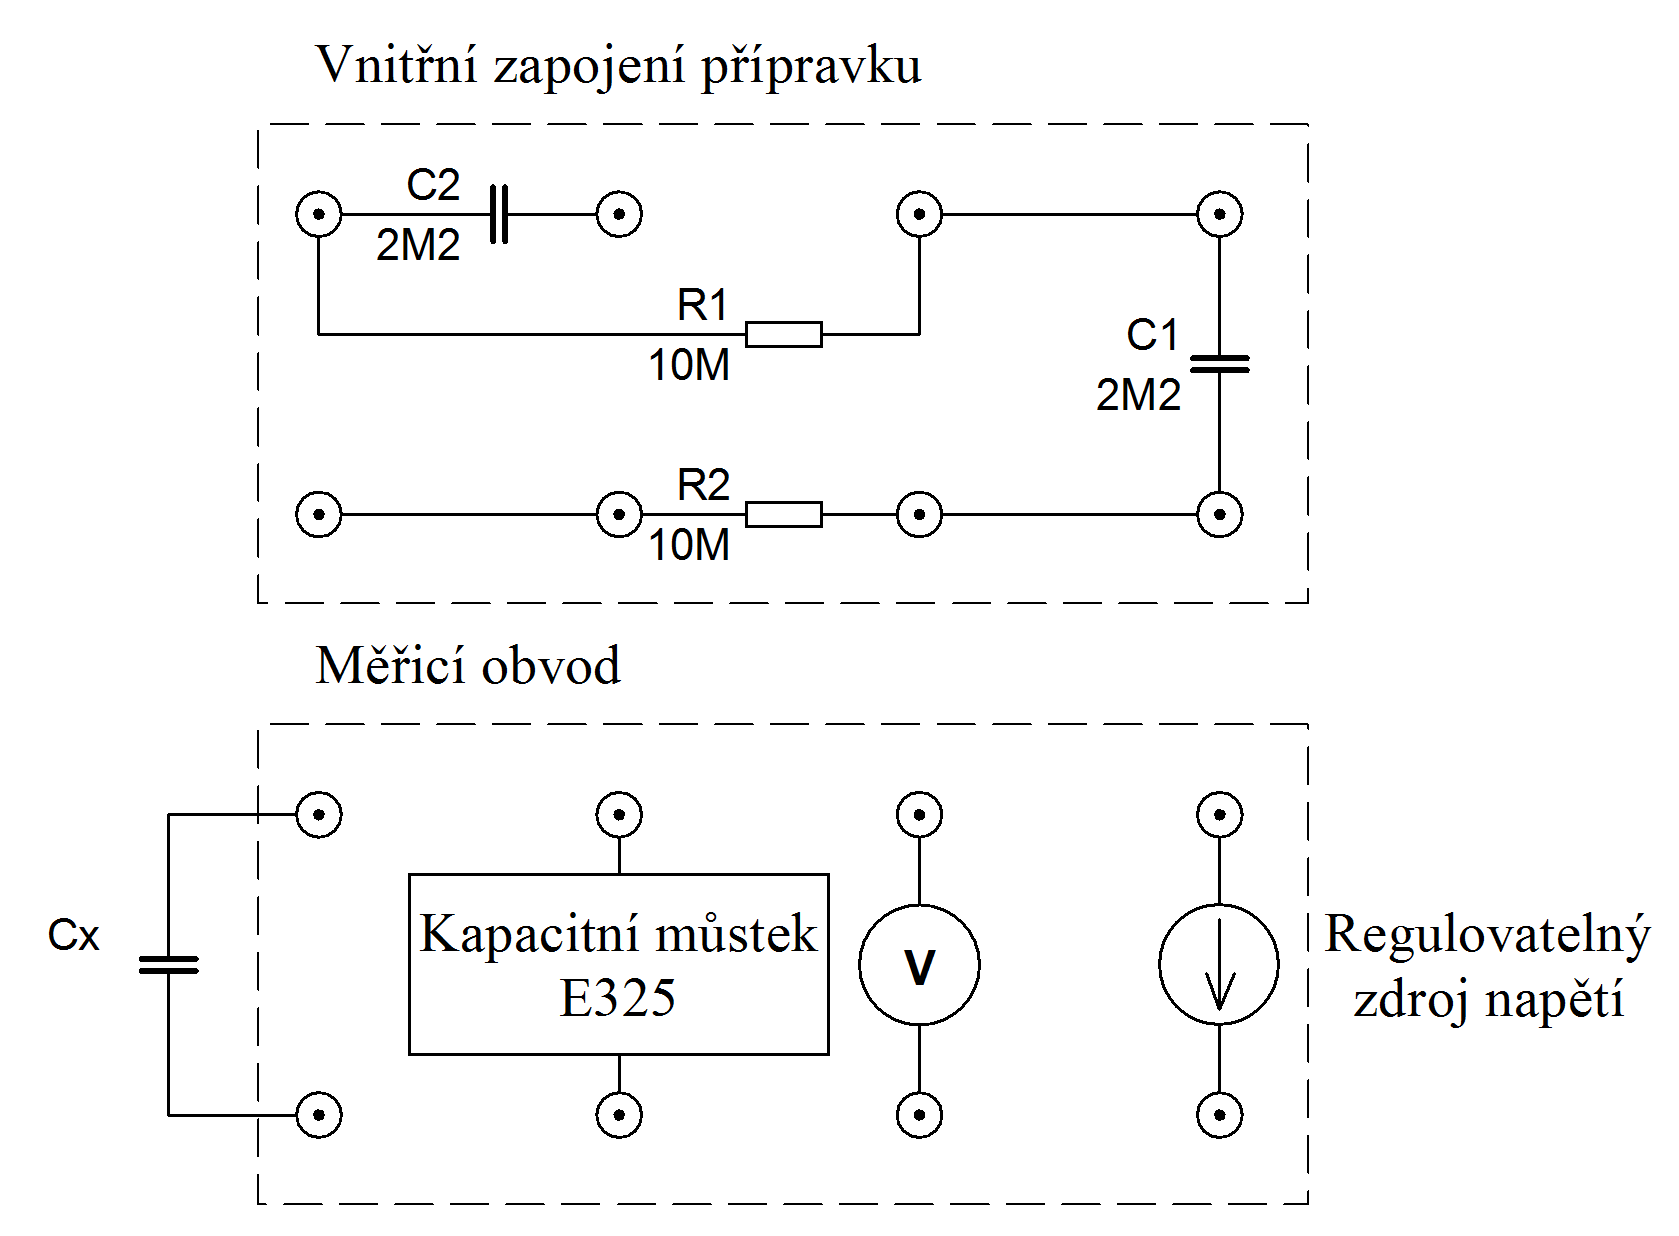
\includegraphics[width=0.7\columnwidth]{feroel_kondenzatory/feroelKond2}
  \label{fig:feroelKond:feroelKond2}
\end{figure}

\subsubsection{\texorpdfstring{Postup m��en�}{Postup mereni}}
M��en� vzorky postupn� zapojujeme na svorky \uv{$C_X$} m��ic�ho p��pravku, kter� umo��uje odd�len� p�ilo�en�ho nap�t� (z bateriov�ho DC zdroje) a m��ic�ho mal�ho st��dav�ho nap�t�, kter� vyu��v�me pro m��en� kapacity. P�i m��en� db�me na to, aby nebylo p�ekro�eno jmenovit� provozn� nap�t� vzorku.

\subsubsection{\texorpdfstring{M��en� vzorky}{Merene vzorky}}
\begin{tabular}{ll}
 1.& keramick� kondenz�tor TK666, 40 V,100 nF, hmota Supermit (kotou�ov�, hn�d�) \\
 2.& keramick� kondenz�tor 4H30, 40 V, 33 nF (zelen�) \\
 3.& svitkov� kondenz�tor CF2, 63 V, 100 nF, tereftal�tov� (�lut�) \\ 
\end{tabular}

%--------------------------------------
\newpage
\subsection{\texorpdfstring{M��en� uvoln�n� n�boje feroelektrick�ho kondenz�toru}{Mereni uvolneni naboje feroelektrickeho kondenzatoru}}
V objemu dielektrika feroelektrick�ho kondenz�toru je obecn� v�dy v�z�n mal� zbytkov� n�boj $Q_1$. Jemu odpov�d� n�zk� nap�t� $U_1$ na svork�ch kondenz�toru, kter� je d�no rovnic�: 

\begin{equation}
U_1 = \frac{Q_1}{C_1}
\label{eq:feroelKond:NapetiNabojKapacita}
\end{equation}

P�i zv��en� teploty doch�z� u feroelektrik k v�razn�mu zmen�en� jejich kapacity (z $C_1$ na $C_2$) d�ky zmen�en� relativn� permitivity z $\epsilon_{r1}$ na $\epsilon_{r2}$. Aby z�stal zachov�n zbytkov� n�boj ($Q_1 = Q_2$), mus� na kondenz�toru v�razn� vzr�st nap�t� ($U_2$). V ide�ln�m p��pad� plat�, �e vzr�st nap�t� ($U_2/U_1$) je roven zm�n� permitivity ($\epsilon_{r1}/\epsilon_{r2}$).

\subsubsection{\texorpdfstring{�kol m��en�}{Ukol mereni}}
Ov��te uvoln�n� elektrick�ho n�boje u p�edlo�en�ho vzorku kondenz�toru z feroelektrick�ho materi�lu.

\subsubsection{\texorpdfstring{Postup m��en�}{Postup mereni}}
Kondenz�tor p�ipojen� k elektrostatick�mu voltmetru nabijte na pln� nap�t� bateriov�ho zdroje (asi 120~V). Kondenz�tor vybijte a po chv�li oh�ejte v olejov� l�zni na cca 150~$^\circ$C. Ode�t�te maxim�ln� nap�t� kondenz�toru.

\section{\texorpdfstring{Vlastnosti vysokofrekven�n�ch c�vek}{Vlastnosti vysokofrekvencnich civek}}

\subsection{\texorpdfstring{�vod}{Uvod}}
Induk�nost v elektrick�m obvodu je obvykle realizov�na c�vkou, tj. uspo��d�n�m vodi�� ve tvaru z�vit�. C�vka m��e b�t navinuta z vodi�� obvykle kruhov�ho pr��ezu do v�lcov�ho nebo diskov�ho tvaru nebo nap�. vytvo�ena jako obrazec na desce plo�n�ch spoj�. Induk�nost c�vky z�vis� na po�tu z�vit�, rozm�rech vinut�, vz�jemn� poloze z�vit� a na magnetick� vodivosti prost�ed�, kter�m se uzav�raj� silo��ry magnetick�ho toku c�vky (vzduch, ferromagnetick� materi�l). P�i pou�it� c�vky v obvodech s vysok�mi frekvencemi nap�t� se v�razn� uplatn� tak� odpor a kapacity vinut�, skinefekt a vf. vlastnosti magnetick�ch materi�l�.

\subsubsection{\texorpdfstring{�initel jakosti - p�ev��en�}{Cinitel jakosti}}

Narozd�l od kondenz�tor� nelze u c�vek zanedbat parazitn� s�riov� odpor. Jen ve velmi ojedin�l�ch p��padech nen� t�eba p�i konstrukci obvodu hodnotu tohoto odporu uva�ovat, nebo� je hlavn� p���inou vzniku ztr�t a z toho plynouc�ho oh�evu c�vky (Jouleovy ztr�ty ve vinut�, ztr�ty v mag. obvodu atd.). �initel jakosti je definov�n jen v rezonan�n�ch obvodech. Zde ud�v� pom�r akumulovan� energie ku ztracen� energii.

P�i s�riov�m spojen� kondenz�toru a c�vky vznikne rezonan�n� obvod, jeho� energie se ztr�c� p�edev��m na parazitn�m odporu c�vky. Rezonan�n� $LC$ obvod tak p�ech�z� na rezonan�n� $RLC$ obvod. �bytek nap�t� na odporu je �m�rn� ztr�t�m v obvodu a nap�t� na induk�nosti (resp. kapacit�) je �m�rn� jalov�mu v�konu, tud� jde o energii akumulovanou v rezonan�n�m obvodu. Anal�zou tohoto faktu z�sk�me pro �initel jakosti vztah:

\begin{equation}
Q= \frac{\omega L}{R}
\label{eq:vfCivky:Q}
\end{equation}

Z�ejm� m��eme �initel jakosti uva�ovat jako p�evr�cenou hodnotu ztr�tov�ho �initele nebo jako pom�r imagin�rn� a re�ln� ��sti impedance c�vky. Jeliko� je odpor c�vky relativn� mal�, dosahuje �initel jakosti na frekvenc�ch ��dov� kHz hodnot ��dov� des�tek a� stovek.

\subsubsection{\texorpdfstring{Nap�t� na prvc�ch v rezonanci}{Napeti na prvcich v rezonanci}}

B�hem rezonance s�riov�ho $RLC$ obvodu doch�z� ke zv��en� amplitudy nap�t� na c�vce a kondenz�toru. Anal�zou vztah� pro impedanci a nap�t� na jednotliv�ch prvc�ch lze odvodit p�vod tohoto jevu. Zde celou v�c zjednodu��me �vahou. P�i rezonanci plat�, �e induktivn� reaktance c�vky je a� na znam�nko rovna kapacitn� reaktanci kondenz�toru. Jejich sou�et je nulov� a impedance obvodu m� pouze re�lnou ��st danou hodnotou odporu. Pro f�zor proudu tak z�sk�v�me vztah:

\begin{equation}
\widehat{I}= \frac{\widehat{U}}{\widehat{Z}}= \frac{\widehat{U}}{\widehat{R}}
\label{eq:vfCivky:Proud}
\end{equation}

Reaktance c�vky a kondenz�toru je st�le v obvodu p��tomna a proch�zej�c� proud vyvol� na obou prvc�ch nap�t�, kter� budou vz�jemn� v protif�zi (v��i sob� posunuta o 180$^\circ$):

\begin{equation}
\widehat{U}_L= \widehat{I}\cdot jX_L= \widehat{U} \cdot \frac{j\omega L}{R} = \widehat{U} \cdot jQ
\label{eq:vfCivky:napetiNaL}
\end{equation}

\begin{equation}
\widehat{U}_C= \widehat{I}\cdot (-jX_C)= \widehat{U} \cdot \frac{-j}{\omega CR} = \widehat{U} \cdot (-jQ)
\label{eq:vfCivky:napetiNaC}
\end{equation}

Z rovnic vypl�v� (\ref{eq:vfCivky:napetiNaL}) a (\ref{eq:vfCivky:napetiNaC}), �e v�sledn� nap�t� na obou reaktanc�ch bude zes�leno velikost� �initele jakosti.

%--------------------------------------
\newpage
\subsection{\texorpdfstring{M��en� frekven�n� z�vislosti �initele p�ev��en� Q}{Mereni frekvencni zavislosti cinitele previseni Q}}

\subsubsection{\texorpdfstring{�kol m��en�}{Ukol mereni}}
Zjist�te m��en�m kmito�tov� z�vislosti �initele p�ev��en� $Q$ dan�ch vzork� c�vek vliv konstruk�n�ho proveden� (d�lky vinut�, rozm�r� a formy vodi��) na jejich kvalitu. Nam��en� hodnoty vyneste do grafu! Diskutujte vliv proveden� vinut� na vlastnosti c�vky. Ov��te vliv feritov�ho j�dra na vlastnosti c�vek.

\subsubsection{\texorpdfstring{Sch�ma zapojen�}{Schema zapojeni}}

\begin{figure}[h]
  \centering
  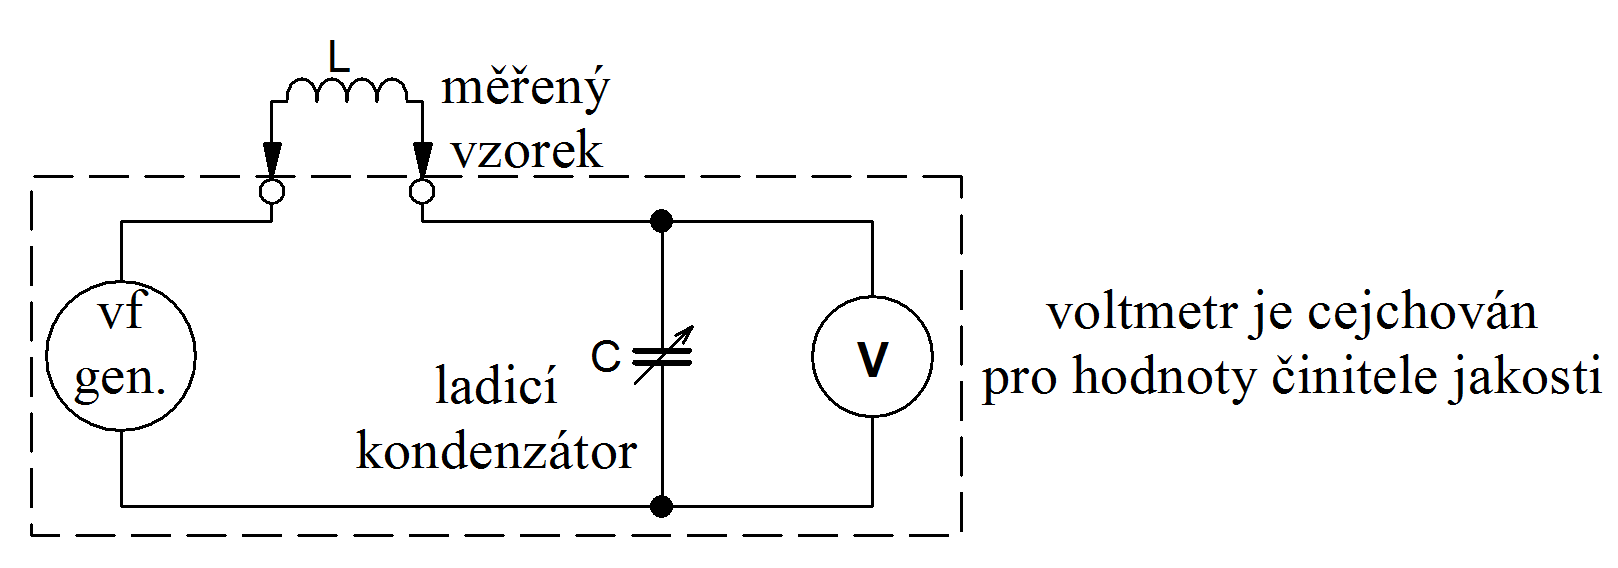
\includegraphics[width=0.7\columnwidth]{vf_civky/vfCivky}
  \label{fig:vfCivky:vfCivky}
\end{figure}

\subsubsection{\texorpdfstring{Postup m��en�}{Postup mereni}}
M��te na Q-metru v kmito�tov�m rozsahu ur�en�m nejmen�� a nejv�t�� kapacitou ladic�ho kondenz�toru p��stroje (obvod s c�vkou se lad� do rezonance).
Kmito�tov� krok volte tak, abyste u ka�d� c�vky zm��ili alespo� 5 hodnot rovnom�rn� rozlo�en�ch v kmito�tov�m intervalu. Vlo�en�m feritov�ho j�dra do c�vek 1 a� 3 (vzorky 4-6) zjist�te zm�nu jejich el. parametr�.

\subsubsection{\texorpdfstring{M��en� vzorky}{Merene vzorky}}
\begin{tabular}{ll}
 1.& c�vka D = 40 mm, l = 27 mm, 13 z�vit� vodi�em $\diameter$ 1,2 mm \\
 2.& c�vka D = 40 mm, l = 27 mm, 27 z�vit� vodi�em $\diameter$ 0,6 mm \\
 3.& c�vka D = 40 mm, l = 27 mm, 57 z�vit� vodi�em $\diameter$ 0,3 mm \\ 
 4.& c�vka D = 40 mm, l = 27 mm, 13 z�vit� vodi�em $\diameter$ 1,2 mm, feritov� j�dro z mat. N1 \\
 5.& c�vka D = 40 mm, l = 27 mm, 27 z�vit� vodi�em $\diameter$ 0,6 mm, feritov� j�dro z mat. N1 \\
 6.& c�vka D = 40 mm, l = 27 mm, 57 z�vit� vodi�em $\diameter$ 0,3 mm, feritov� j�dro z mat. N1 \\
 7.& c�vka MESC (GES Electronic), 10 $\mu$H, feritov� j�dro ty�inka \\
 8.& c�vka 09P (GM Electronic), 560 $\mu$H, feritov� j�dro c�vka \\
\end{tabular}

%--------------------------------------
\newpage
\subsection{\texorpdfstring{M��en� frekven�n� z�vislosti induk�nosti $L_S$ a �initele p�ev��en� $Q$ vzork� na feritov�ch j�drech}{Mereni frekvencni zavislosti indukcnosti Ls}}

\subsubsection{\texorpdfstring{�kol m��en�}{Ukol mereni}}
Zm��te s�riovou induk�nost LS a �initel p�ev��en� Q v z�vislosti na frekvenci. Najd�te frekvenci pro maxim�ln� hodnotu Q a frekvenci vlastn� rezonance fr. M��en� prove�te pomoc� LCR metru HP4284A.

\subsubsection{\texorpdfstring{Postup m��en�}{Postup mereni}}
M��te na Q-metru v kmito�tov�m rozsahu ur�en�m nejmen�� a nejv�t�� kapacitou ladic�ho kondenz�toru p��stroje (obvod s c�vkou se lad� do rezonance).
Kmito�tov� krok volte tak, abyste u ka�d� c�vky zm��ili alespo� 5 hodnot rovnom�rn� rozlo�en�ch v kmito�tov�m intervalu. Vlo�en�m feritov�ho j�dra do c�vek 1 a� 3 (vzorky 4-6) zjist�te zm�nu jejich el. parametr�.

\subsubsection{\texorpdfstring{M��en� vzorky}{Merene vzorky}}
\begin{tabular}{ll}
 1.& tlumivka 3,7 mH (feritov� j�dro obd�ln�kov�) \\
 2.& tlumivka 600 $\mu$H (feritov� j�dro obd�ln�kov�) \\
\end{tabular}

%--------------------------------------
\subsection{\texorpdfstring{Obr�zkov� p��loha}{Obrazkova priloha}}

\begin{figure}[h]
  \centering
  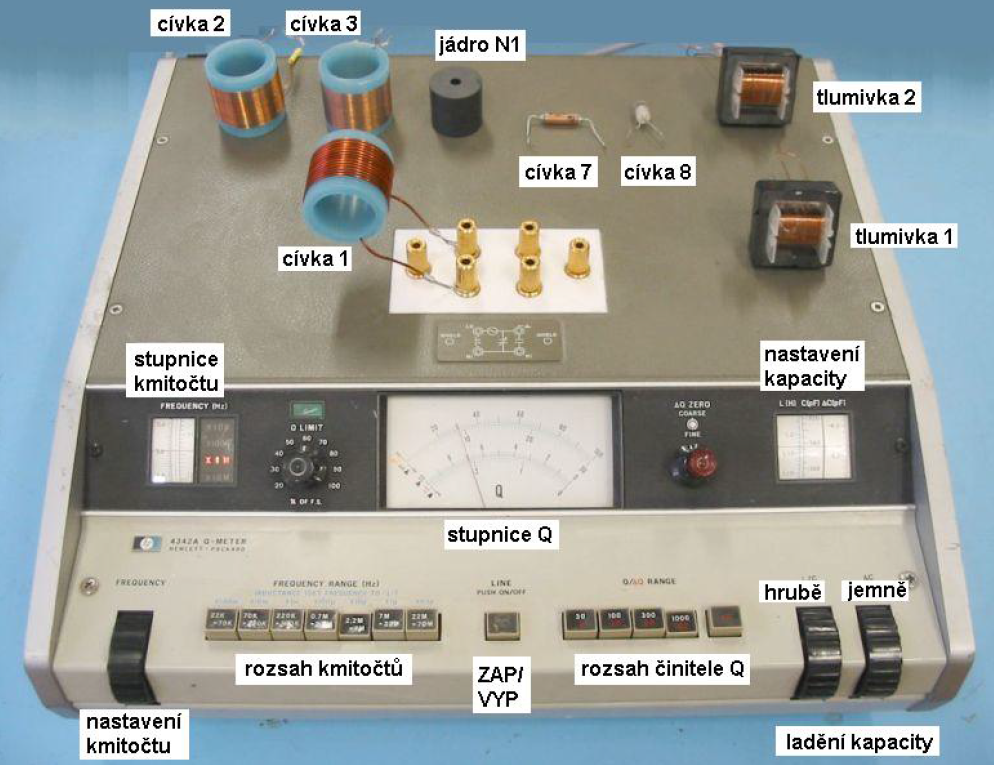
\includegraphics[width=0.9\columnwidth]{vf_civky/qmetr}
  \label{fig:vfCivky:qmetr}
\end{figure}
\section{\texorpdfstring{Osazov�n� DPS}{Osazovani DPS}}

\subsection{\texorpdfstring{�vod}{Uvod}}
P�jen� je zp�sob spojov�n� dvou kovov�ch materi�l� pomoc� jin�ho roztaven�ho kovov�ho materi�lu, tzv. p�jky. Teplota t�n� p�jky je obvykle mnohem ni���, ne� je tomu u p�jen�ch materi�l�, proto p�i p�jen� nedoch�z� k taven� spojovan�ch sou��st�. V elektrotechnice se pro vytv��en� vodiv�ch spoj� pou��vaj� t�m�� v�hradn� tzv. m�kk� p�jky. To jsou materi�ly, u nich� je teplota t�n� ni��� ne� 400~$^\circ$C. Lze se setkat se dv�ma skupinami pou��van�ch slitin:
P�jky obsahuj�c� olovo � jsou zalo�eny na slitin� Sn-Pb. Jejich v�hodou je n�zk� bod t�n�, kter� je pouze 183~$^\circ$C. Nev�hodou je obsah olova, kter� je toxick�. Pou��v�n� t�chto p�jek je omezeno sm�rnic� RoHS pouze pro speci�ln� ��ely.
P�jky bez olova � jde o slitiny c�nu a dal��ch kov�, jako nap��klad Ag, Zn, Cu a dal��. Teplota t�n� je vy��� ne� u p�jek s olovem a jej� obvykl� hodnota je 217~$^\circ$C.
Tavidla jsou nekovov� materi�ly usnad�uj�c� p�jen�. Zlep�uj� sm��ivost dan�ch materi�l� p�jkou a br�n� oxidaci roztaven� p�jky. Nej�ast�ji se pro tento ��el pou��v� kalafuna.

%--------------------------------------
\newpage
\subsection{\texorpdfstring{Osazov�n� desky plo�n�ho spoje}{Mereni frekvencni zavislosti cinitele previseni Q}}

\subsubsection{\texorpdfstring{�kol m��en�}{Ukol mereni}}
Osa�te p�ipraven� plo�n� spoj a pomoc� p��pravku ov��te jeho funk�nost.

\subsubsection{\texorpdfstring{Popis zapojen�}{Popis zapojeni}}
Sch�ma zapojen� osazovan�ho obvodu je na obr�zku \ref{fig:osDPS:schemaZap}. Jedn� se o akustickou signalizaci, kter� m� upozornit �idi�e na nutnost rozsv�tit sv�tla. Nap�jec� nap�t� a logick� sign�ly sv�tel jsou p�iv�d�ny na konektor K1. Reproduktor je p�ipojen mezi v�vody J1 a J2. Ke generov�n� obd�ln�kov�ho sign�lu pro reproduktor je pou�it integrovan� obvod �asova�e TS555. Sign�l je odeb�r�n proti zemi z v�stupu Q. Hodnotu periody generovan�ho sign�lu lze ovlivnit zm�nou �asov� konstanty RC �l�nku, kter� je slo�en z rezistoru R1 a kondenz�toru C3.
�innost �asova�e je ovliv�ov�na logickou �rovn� na vstupu R. Pokud je zde n�zk� �rove�, pak je �asova� vy�azen z �innosti. Po p�ipojen� nap�jec�ho nap�t� (oto�en� kl��ku automobilu) je na tomto vstupu nap�t� bl�zk� 0 V d�ky rezistoru R2, kter� je p�ipojen proti plovouc� zemi (bude vysv�tleno d�le). �asova� tedy nekmit�, dokud nap�t� na tomto vstupu nedos�hne po�adovan� vysok� �rovn�. Nap�t� je na vstup p�iv�d�no p�es diodu D5 z kondenz�toru C2, kter� je pozvolna nab�jen z nap�jec�ho zdroje p�es diodu D3 a rezistor R4. Volbou hodnot rezistoru R4 a kondenz�toru C2 tak ovliv�ujeme d�lku �asov� prodlevy p�ed spu�t�n�m akustick� signalizace po zapnut� p��pravku.
Nap�jec� nap�t� pro �asova� je vyvedeno mezi uzly V+ a GND. GND je zde zna�ena plovouc� zem, co� je uzel, kter� je odd�len od skute�n� zem� nap�jec�ho zdroje rezistorem R5. P�iveden�m ur�it�ho nap�t� na tento rezistor p�es diody D1 nebo D2 sn��me o jeho hodnotu nap�jec� nap�t� �asova�e. Pokud je toto nap�t� rovno nap�t� zdroje nap�jen�, pak je nap�jec� nap�t� �asova�e rovno nule a obvod op�t nem��e kmitat.

\subsubsection{\texorpdfstring{Postup p�jeni}{Postup pajeni}}
Desku plo�n�ho spoje osazujeme dle obr�zku \ref{fig:osDPS:schemaPokl}, kter� ukazuje pozice sou��stek ze strany sou��stek (druh� strana se naz�v� strana plo�n�ho spoje a jsou na n� vyleptan� vodiv� trasy). Db�me na polaritu diod a elektrolytick�ch kondenz�tor� a tak� na spr�vn� nato�en� pouzdra integrovan�ho obvodu, kter� je vyzna�eno kl��em (symbol na pouzd�e � te�ka, v��ez apod.). P�i osazov�n� je vhodn� za��t sou��stkami s n�zk�m profilem (v��kou). P�jen� bude jednodu���, pokud si desku plo�n�ho spoje upevn�me do dr��ku.
\noindent
Spoje p�j�me n�sleduj�c�m posupem:
\begin{enumerate}
	\item P�je�ku dr��me v jedn� ruce, trubi�kovou p�jku ve druh�.
	\item P�ilo��me p�je�ku ke spoji a za�neme jej proh��vat (p��padn� je�t� p�edt�m namo��me p�je�ku do kalafuny).
	\item Dotkneme se p�jkou proh��van�ho spoje � trocha p�jky se roztav� a z�stane na p�je�ce a spoji. P�je�kou st�le proh��v�me spoj!!!
	\item Pot� co se p�jka rozte�e po spoji, p�je�ku odejmeme. V�dy se sna��me, zkr�tit dobu p�jen� na minimum.
\end{enumerate}
V�sledn� p�jen� spoj by m�l m�t vzhled sopky.
\newpage
\subsubsection{\texorpdfstring{Sch�ma zapojen�}{Sch�ma zapojen�}}

\begin{figure}[h]
  \centering
  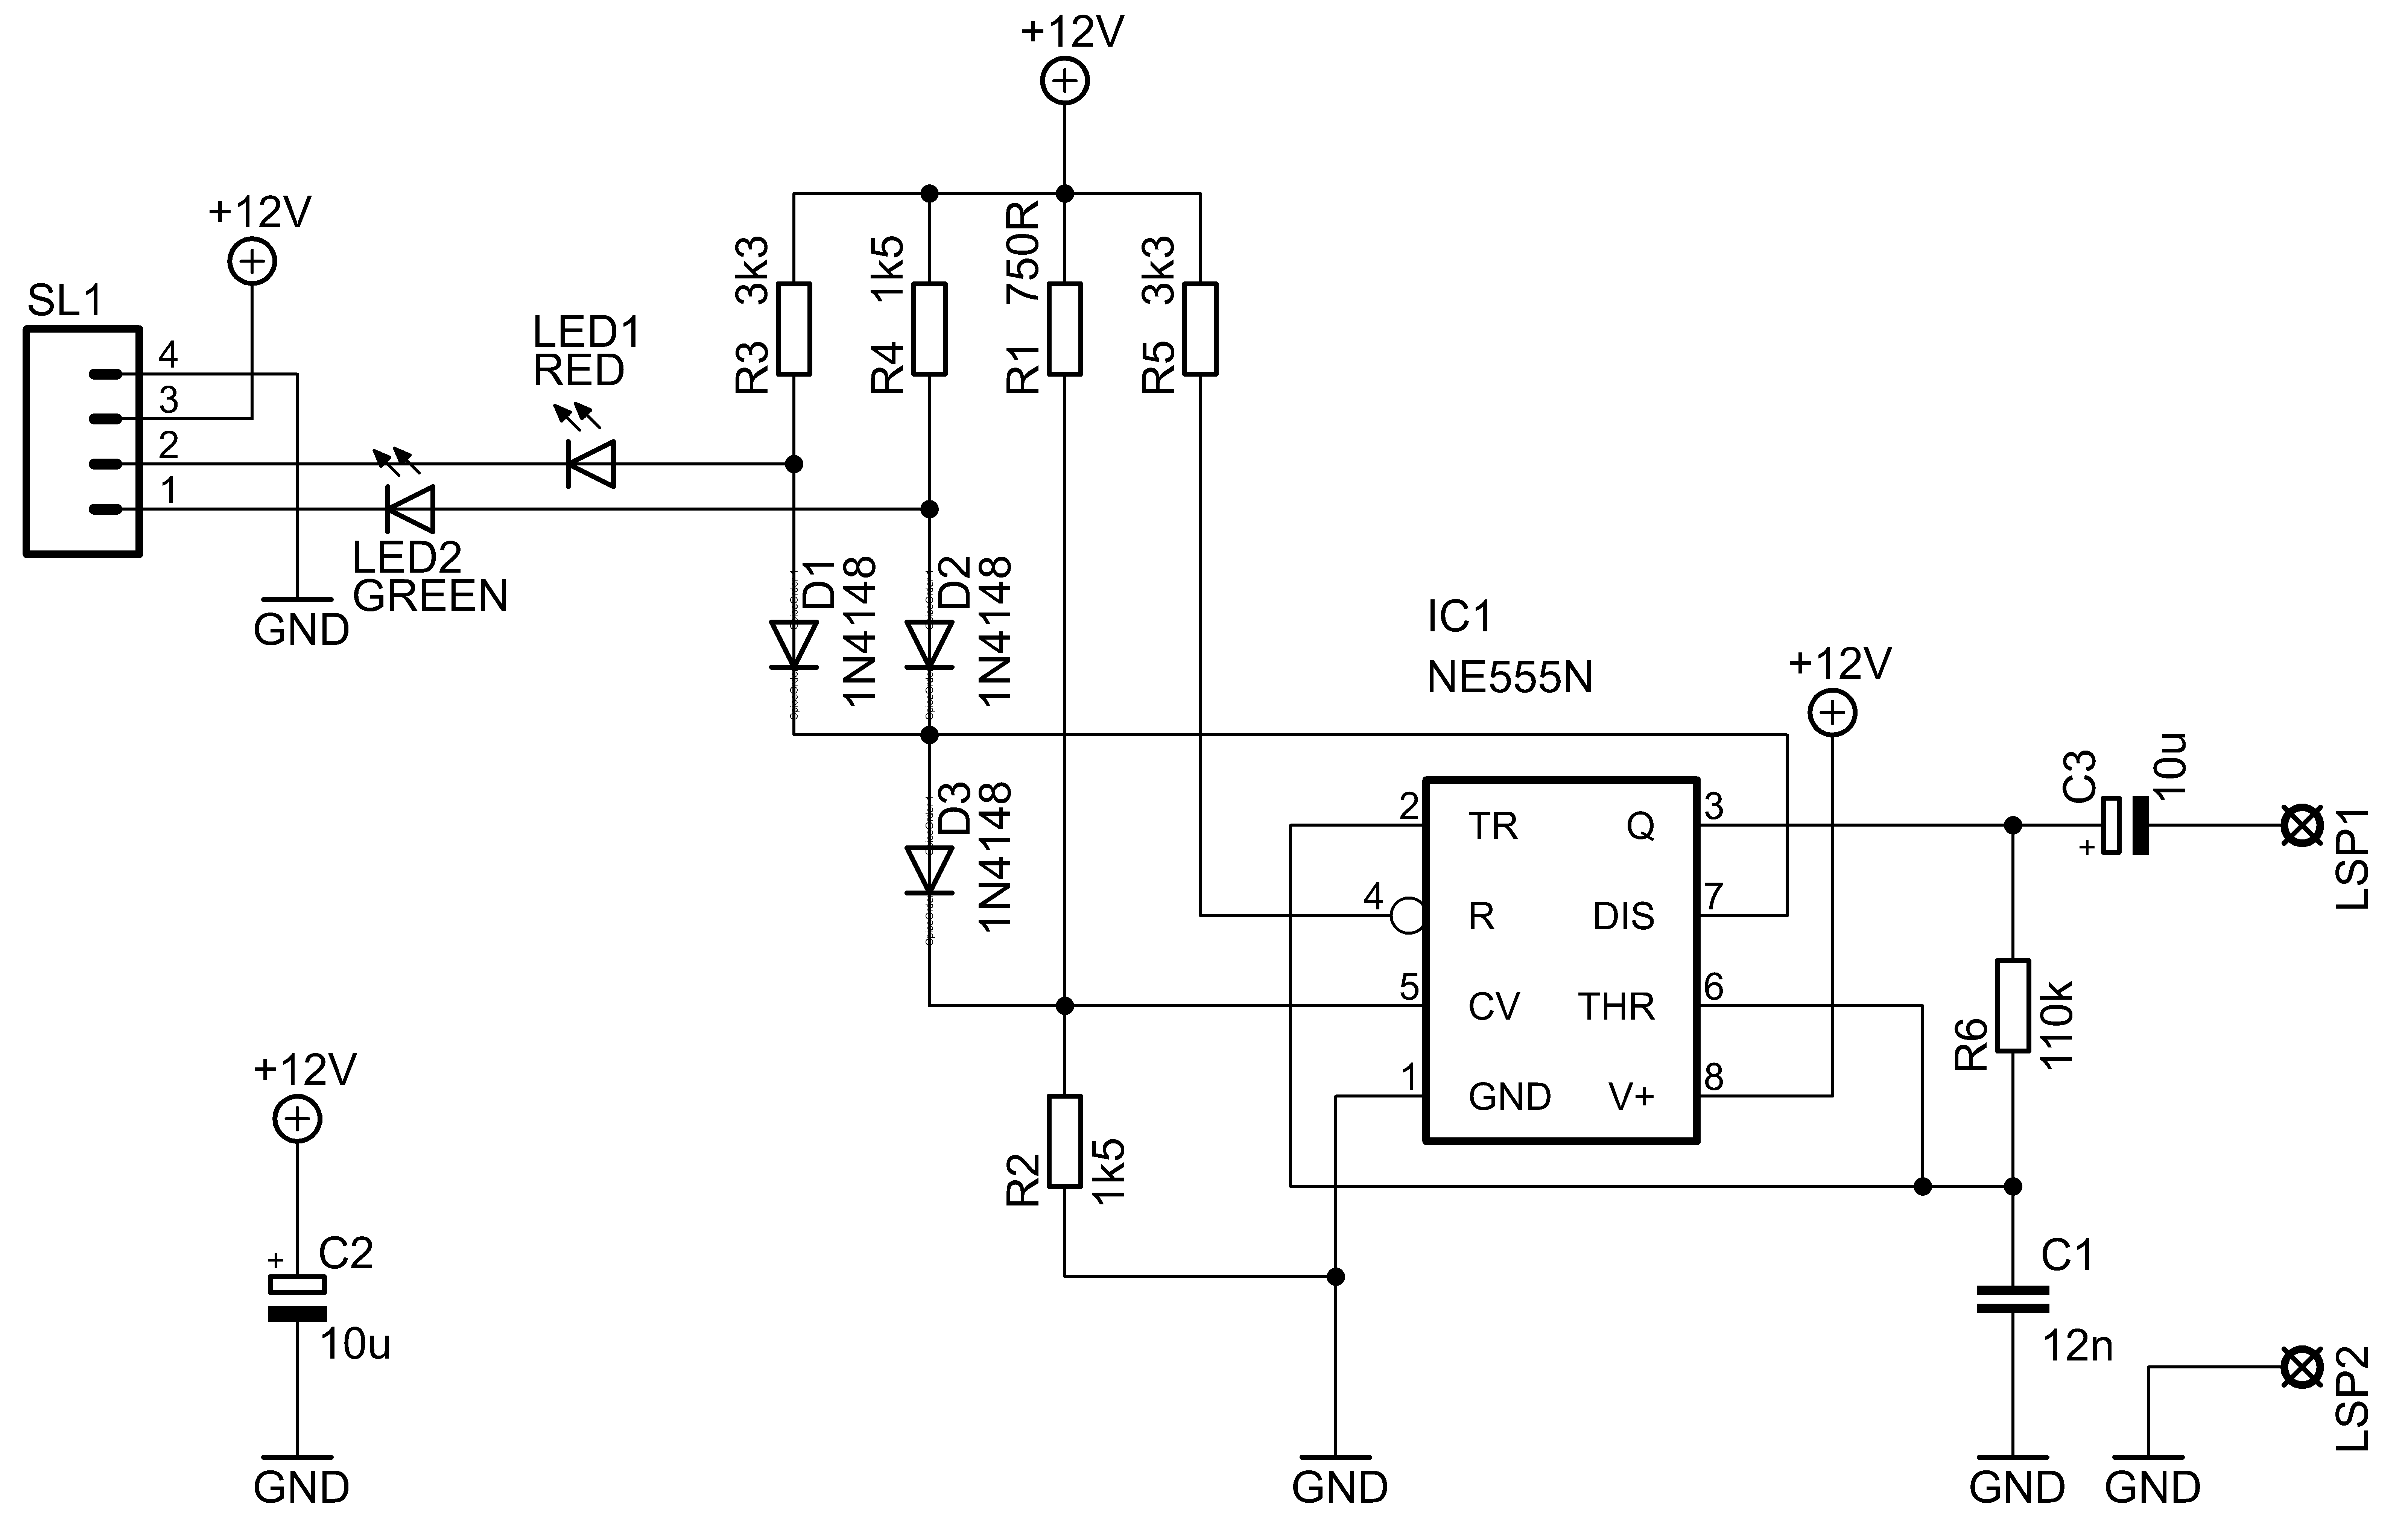
\includegraphics[width=0.8\columnwidth]{osazovani_dps/svetla_piskle_schema}
	\caption{Sch�ma zapojen� signalizace rozsv�cen�ch sv�tel}
  \label{fig:osDPS:schemaZap}
\end{figure}

\begin{figure}[h]
  \centering
  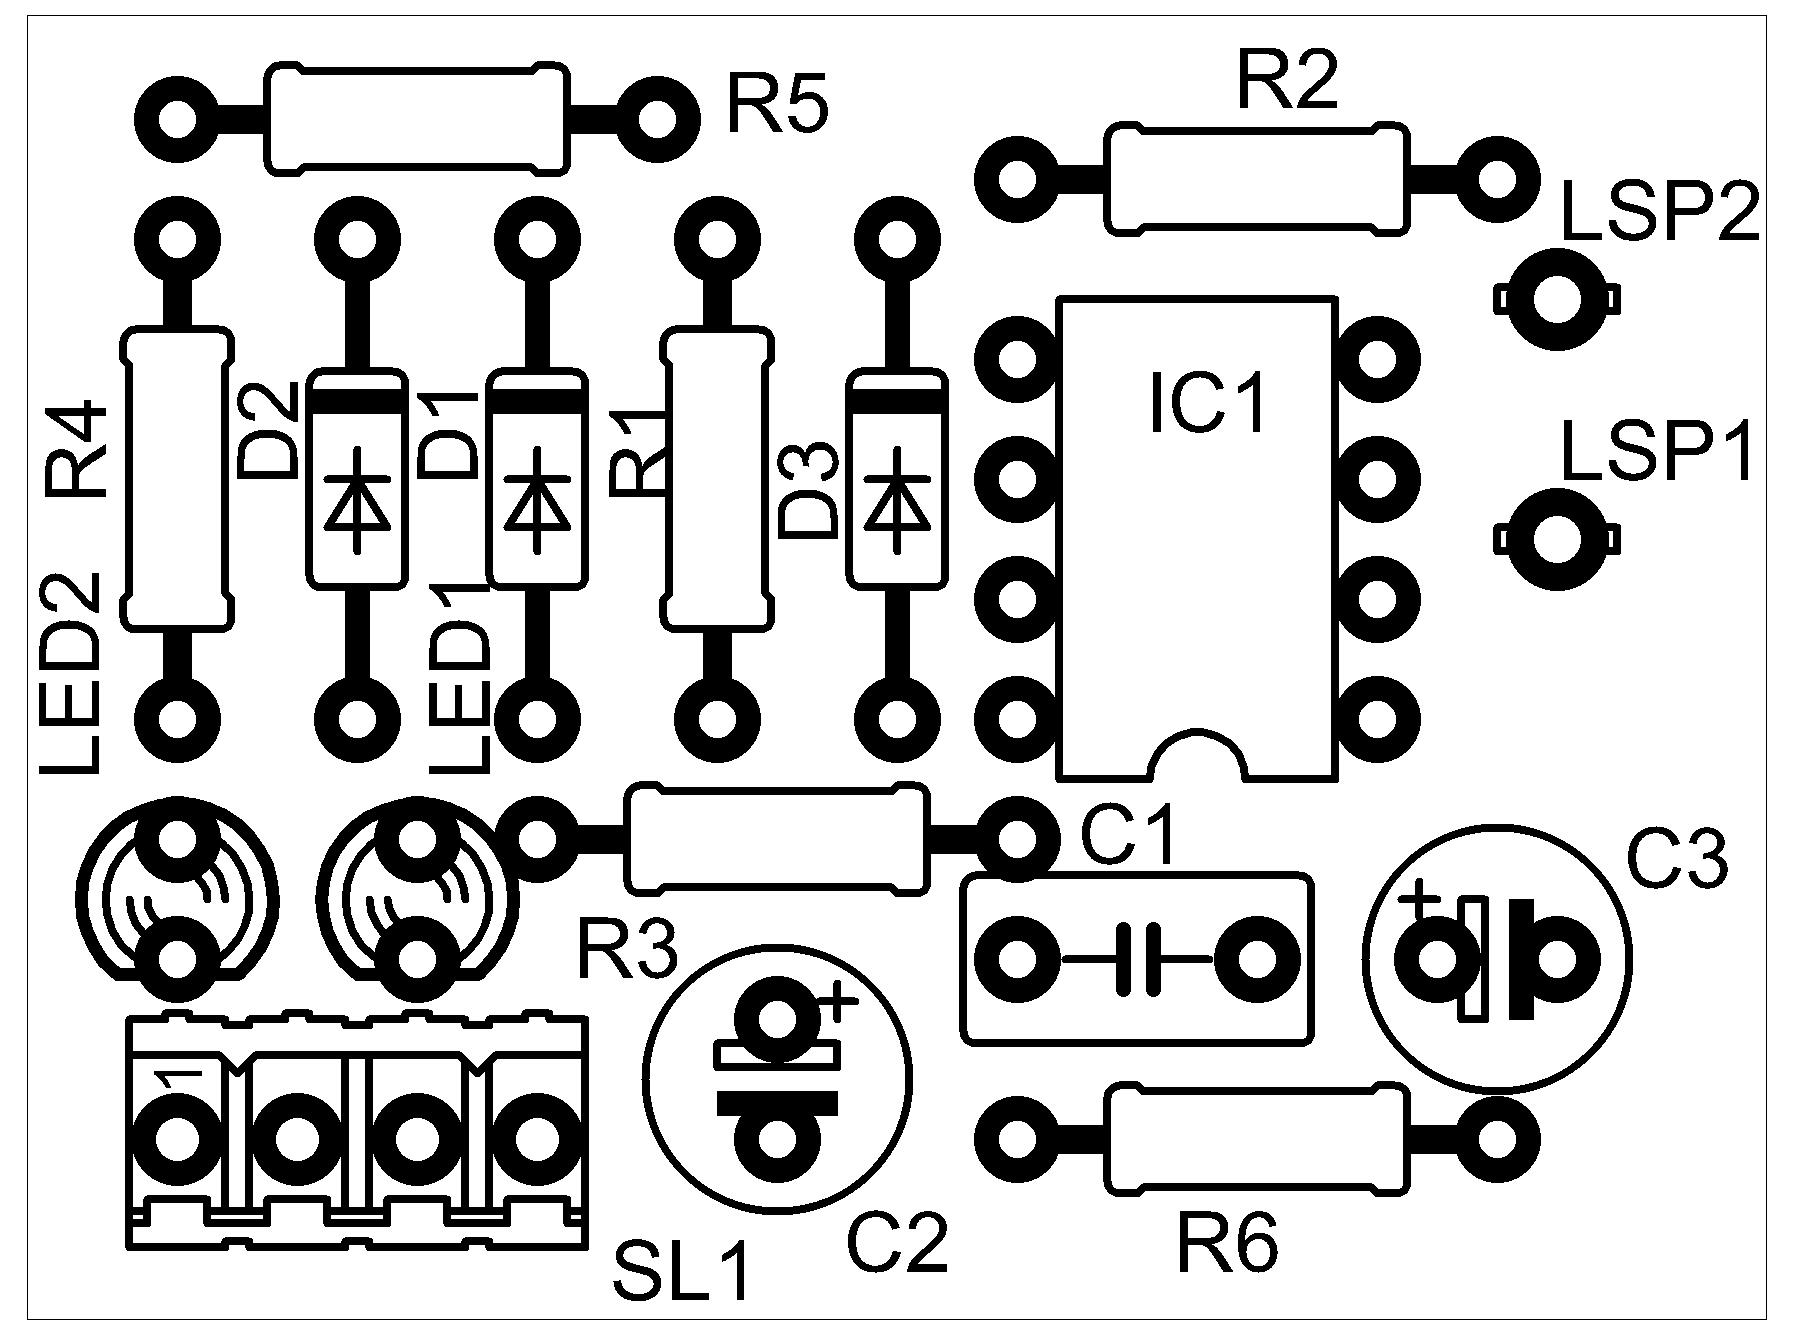
\includegraphics[width=0.4\columnwidth]{osazovani_dps/piskle_S}
	\caption{Pokl�dac� (osazovac�) sch�ma}
  \label{fig:osDPS:schemaPokl}
\end{figure}

\subsubsection{\texorpdfstring{Zna�en� rezistor�}{Znaceni rezistoru}}

\begin{center}
\begin{tabular}{|l|c|c|c|c|c|}
\hline
 Barva & 1. pruh & 2. pruh & 3. pruh & N�sobitel & Tolerance \\
\hline
 �ern� & 0 & 0 & 0 & 1 &\\
 hn�d� & 1 & 1 & 1 & 10 & 1\% \\
 �erven� & 2 & 2 & 2 & 100 & 2\% \\
 oran�ov� & 3 & 3 & 3 & $10^3$ & \\
 �lut� & 4 & 4 & 4 & $10^4$ & \\
 zelen� & 5 & 5 & 5 & $10^5$ & 0,5\% \\
 modr� & 6 & 6 & 6 & $10^6$ & 0,25\%\\
 fialov� & 7 & 7 & 7 & $10^7$ & 0,1\% \\
 �ed� & 8 & 8 & 8 & $10^8$ & 0,05\%\\
 b�l� & 9 & 9 & 9 & $10^9$ & \\
 zlat� &&&& 0,1 & 5\%\\
 st��brn� &&&& 0,01 & 10\%\\
\hline
\end{tabular}
\end{center}
\section{\texorpdfstring{Vlastnosti kondenz�tor� a rezistor� p�i kmito�tech nad 1~MHz }{Vlastnosti kondenzatoru a rezistoru pri kmitoctech nad 1 MHz}}

\subsection{\texorpdfstring{�vod}{Uvod}}

Rezistory a kapacitory nejsou ide�ln� sou��stky, tak�e mimo svou dominantn� vlastnost (odpor, kapacita) vykazuj� je�t� parazitn� vlastnosti (induk�nost, kapacitu, s�riov� a paraleln� odpor). Ty ovliv�uj� jejich vlastnosti, a to p�edev��m v obvodech s vy���mi frekvencemi. M��en� slou�� k ov��en� kmito�tov�ho rozsahu, v n�m� sou��stka vykazuje p�ev�n� svou dominantn� vlastnost. Vlastnosti jednotliv�ch vzork� z�vis� na jejich rozm�rech, pou�it�ch materi�lech, technologii v�roby atd.

%---------------------------------------------
\subsection{\texorpdfstring{Kmito�tov� z�vislost rezistor�}{Kmitoctova zavislost rezistoru}}

\subsubsection{\texorpdfstring{�kol m��en�}{Ukol mereni}}
Pro zadan� vzorky rezistor� zm��te z�vislost absolutn� hodnoty impedance a f�ze ($\left|Z\right|$, $\varphi$) na kmito�tu. Nam��en� hodnoty vyneste do grafu. V z�v�ru diskutujte vliv hodnoty a technologie rezistoru na nam��en� frekven�n� charakteristiky.

\subsubsection{\texorpdfstring{Postup m��en�}{Postup mereni}}

M��en� prove�te v rozsahu frekvenc� 1 MHz a� 100 MHz s pou�it�m p��stroje Agilent E5062A. Vyhodno�te, jak se jednotliv� vzorky projevuj� v z�vislosti na jejich hodnot� a technologii. Zaznamenejte rezonan�n� frekvence jednotliv�ch sou��stek.

\subsubsection{\texorpdfstring{M��en� vzorky}{Merene vzorky}}
\begin{tabular}{lll}
 1.& 10~$\Omega$/ 330~$\Omega$/ 10~k$\Omega$& rezistor metalizovan�, 0,6 W, velikost 0207  \\
 2.& 10~$\Omega$/ 330~$\Omega$/ 10~k$\Omega$& rezistor metalizovan�, 2 W  \\
 3.& 10~$\Omega$/ 330~$\Omega$/ 10~k$\Omega$& rezistor dr�tov�, 5 W  \\ 
\end{tabular}

%---------------------------------------------
\subsection{\texorpdfstring{Kmito�tov� z�vislost kondenz�tor�}{Kmitoctova zavislost kondenzatoru}}

\subsubsection{\texorpdfstring{�kol m��en�}{Ukol mereni}}
Pro zadan� vzorky kondenz�tor� zm��te z�vislost kapacity a ztr�tov�ho �initele ($C$, $tg\delta$) na kmito�tu. Nam��en� hodnoty vyneste do grafu. V z�v�ru diskutujte vliv technologie kondenz�toru na nam��en� frekven�n� charakteristiky.

\subsubsection{\texorpdfstring{Postup m��en�}{Postup mereni}}

M��en� prove�te v rozsahu frekvenc� 1~MHz a� 100~MHz s pou�it�m p��stroje Agilent E5062A. Vyhodno�te, jak se jednotliv� vzorky projevuj� v z�vislosti na jejich technologii. Zaznamenejte rezonan�n� frekvence jednotliv�ch sou��stek.

\subsubsection{\texorpdfstring{M��en� vzorky}{Merene vzorky}}
\begin{tabular}{llll}
 1.& Elektrolytick� kondenz�tor hlin�kov�, 330 $\mu$F/ 25 V &  5.& Keram. kondenz�tor, 1 nF  \\
 2.& Elektrolytick� kondenz�tor tantalov�, 22 $\mu$F/ 10 V & 6.& Keram. kondenz�tor, 10 nF  \\ 
 3.& Foliov� kondenz�tor radi�ln�, 10 nF/ 100 V  & 7.& Keram. kondenz�tor, 68 nF  \\ 
 4.& Foliov� kondenz�tor axi�ln�, 10 nF/ 100 V  && \\
\end{tabular}

%---------------------------------------------
\subsection{\texorpdfstring{M��en� p��strojem Agilent E5062A}{Mereni pristrojem Agilent E5062A}}

\subsubsection{\texorpdfstring{Sch�ma zapojen�}{Schema zapojeni}}

\begin{figure}[h]
  \centering
  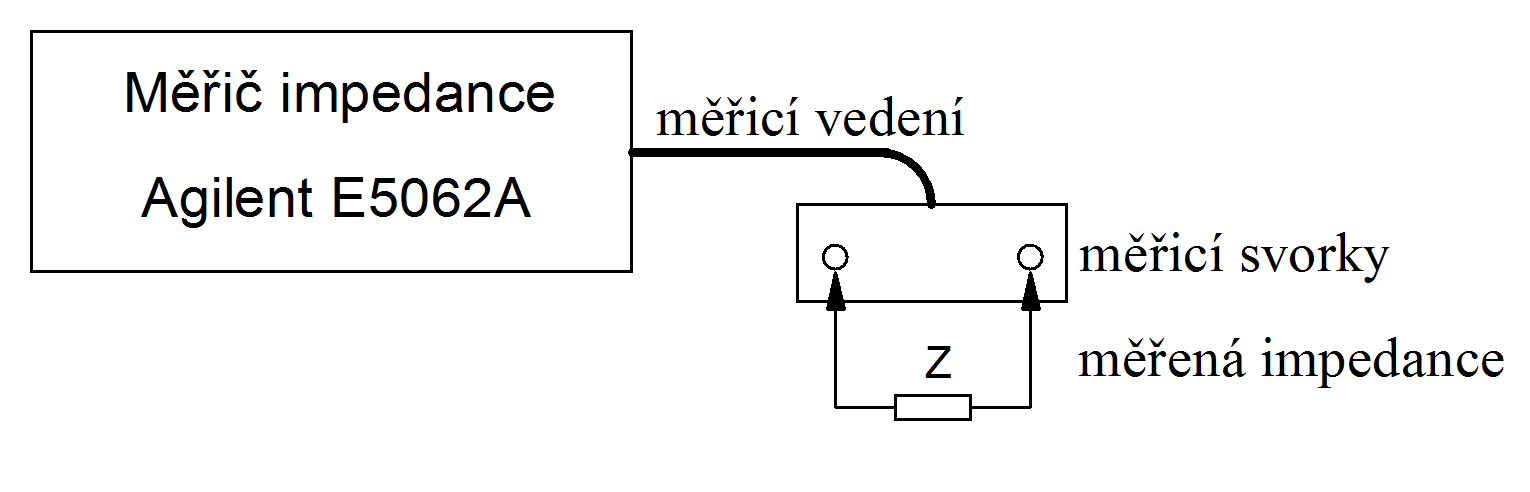
\includegraphics[width=0.2\columnwidth]{rc_nad_1MHz/RCmer21}
  \label{fig:rcNad1MHz:schemaZap}
\end{figure}

\subsubsection{\texorpdfstring{Postup m��en�}{Postup mereni}}
Bez zalo�en�ho vzorku na za��tku m��en� zkontrolujeme kalibraci p��stroje � kurzor ukazuje na prav� okraj kru�nice na displeji (poloha 3 hodiny). Pokud ne, je t�eba kalibrovat:

\textbf{\uv{Save/Recall} / \uv{Recall/State} / \uv{File Dialog} / \uv{Lab.sta} / \uv{Open}} 

\noindent Zalo��me vzorek do �elist�. Tla��tky \textbf{START} a \textbf{STOP} lze zadat z kl�vesnice po��te�n� a kone�nou frekvenci m��en�. Body k�ivky m��eme ��st manu�ln� nebo zaznamenat celou k�ivku automaticky na pam�ov� medium.

\subsubsection*{\texorpdfstring{Manu�ln� nastaven� frekvence:}{Manualni nastaveni frekvence}}
Aktu�ln� frekvenci m��eme nastavit p�i nastaven� volby Marker /Marker1. Frekvenci nastavujeme ot��en�m voli�e nebo z kl�vesnice. Na displeji je mo�n� ode��st �daje v n�sleduj�c�m po�ad�: frekvence ($f$), odpor ($R$), reaktance ($X$), induk�nost ($L$) nebo kapacita ($C$) podle znamenka reaktance.

\subsubsection*{\texorpdfstring{Automatick� m��en�:}{Automaticka mereni}}
M��en� prob�h� kontinu�ln�. Data zapisujeme na flash disk. Postupn� vol�me:

\textbf{\uv{Save/Recall} / \uv{Save Trace Data}}

\noindent \textbf{Nezapome�te zvolit vhodn� ulo�i�t�!!!}. Jm�no souboru je nutn� zadat z kl�vesnice. Stiskem \textbf{\uv{Save}} se data ulo�� ve fotm�tu CSV. Form�t ukl�d�n� je CSV. Tento form�t soubor� lze b�n� editovat softwary Excel, Matlab apod.

\subsubsection{\texorpdfstring{Smith�v diagram}{Smithuv diagram}}
\begin{multicols}{2}

\begin{centering}
  \includegraphics[width=0.8\columnwidth]{rc_nad_1MHz/smithDiag}
  \label{fig:rcNad1MHz:smithDiag}
\end{centering}

Smith�v diagram graficky zn�zor�uje z�vislost �initele odrazu na zakon�ovac� impedanci veden� $Z$.

\begin{equation}
\rho = \frac{Z-Z_0}{Z+Z_0}
\label{eq:rcNad1MHz:cinitelOdrazu}
\end{equation}

P�i zn�m�m �initeli odrazu $\rho$ (lze zm��it) a zn�m� charakteristick� impedanci veden� $Z_0$ lze ze Smithova diagramu ur�it zakon�ovac� impedanci veden�.
\end{multicols}

\end{document}
